\section{Experiments and Results}


This section outlines the experimental setup and evaluates the performance of the proposed PathFinder framework. First, we conduct a qualitative assessment of the descriptions generated by the Description Agent, comparing them to two vision-language models (VLMs). Next, we evaluate PathFinder on the M-Path dataset for melanoma diagnosis (see Section \ref{data-mpath}), benchmarking it against state-of-the-art transformer-based and MIL-based baselines, as well as public and private large language models (LLMs) using prompting without additional training. Finally, we analyze PathFinder's performance under various configurations, altering the Triage, Navigation, and Description Agents. Detailed evaluations are provided in the following subsections.


\subsection{Pathologist Evaluation of Description Quality}
\label{sup:pathologist-analysis}




To assess the quality of descriptions generated by our Description Agent, we conducted a survey in which two expert pathologists rated descriptions produced by our Description agent in comparison to those generated by GPT4-o \cite{hurst2024gpt} and LLaVA-Med \cite{li2024llava}. We selected 25 cases from the M-Path dataset, sampling across the four diagnostic classes. For each case, we cropped the consensus region of interest, manually labeled by a panel of expert dermatopathologists as the area most representative of the diagnosis. Using this region, we prompted our Description Agent, LLaVA-Med and GPT4-o to generate concise descriptions of each histopathology patch. These descriptions were then presented to two expert pathologists in a randomized, double-blind format. Each pathologist was asked to respond to two questions for each case to indicate their preferred description and the reason for their preference. Refer to Appendix \ref{supp:pathologists-analysis} for a detailed explanation of this assessment. The results shown in Figure \ref{fig:pathologist-analysis} indicate that, PathFinder's Description agent achieves comparable performance to GPT-4o while being significantly more cost-effective, operating with just 7B parameters - a fraction of GPT-4o's size.

\begin{figure}[h]
    \centering
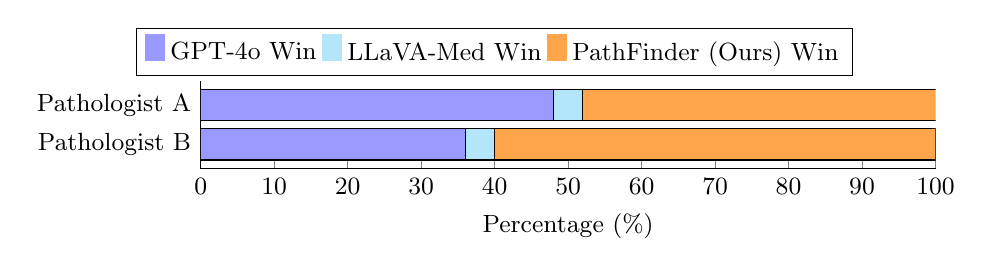
\begin{tikzpicture}
    \begin{axis}[
        width=0.9\linewidth,
        height=2.7cm,
        xbar stacked,
        bar width=0.4cm, % height, because we flipped.
        xmin=0, xmax=100,
        axis x line*=bottom,
        axis y line*=left,
        ymin=-0.2, ymax=1.2, % add some buffer border
        ytick=data,
        yticklabels={Pathologist B, Pathologist A},
        % nodes near coords,
        % nodes near coords align={left},
        enlarge y limits=0.3,
        xlabel={Percentage (\%)},
        % legend style={font=\small, at={(0.4,1.6)}, anchor=north, legend columns=-1},
        tick label style={font=\small}, % Adjust tick labels
        label style={font=\small},      % Adjust axis labels
        legend style={font=\small, at={(0.4,1.6)}, anchor=north, legend columns=-1},
        legend image code/.code={
            \draw[#1, draw=none] (0cm,-0.1cm) rectangle (0.25cm,0.25cm);
        },
    ]
    % A's score label and bars
    \addplot[fill=blue!40] coordinates {(36,0) (48,1)}
        node[anchor=east, xshift=-1em] at (axis cs:0,0) {Pathologist A's score};  % Label for A's score at (36,0)
    
    % B's score label and bars
    \addplot[fill=cyan!30] coordinates {(4.0,0) (4.0,1)}
        node[anchor=east, xshift=-1em] at (axis cs:0,1) {Pathologist B's score};  % Label for B's score at (4,0)
    
    % Additional bars without labels
    \addplot[fill=orange!70] coordinates {(60,0) (48.1,1)};
    
    \legend{GPT-4o Win, LLaVA-Med Win, PathFinder (Ours) Win}
    \end{axis}
\end{tikzpicture}

\caption{Expert human pathologist preferences for each model in assessing description quality, evaluated in a double-blind survey for unbiased comparison.}

\label{fig:pathologist-analysis}
\end{figure}

\subsection{PathFinder Evaluation}





For evaluating PathFinder, we utilize the M-Path dataset which contains histopathology WSIs of melanocytic skin tissue. As outlined in \ref{trajectories}, multiple trajectories are generated per case to simulate the variability in diagnostic patterns observed among pathologists, who may assess a single case with diverse visual strategies to identify diagnostically significant regions. To mitigate randomness in our results, we evaluated PathFinder 10 times on the test set, each time using a different random subset of 5 trajectories selected from the total of 20. For each Whole Slide Image (WSI), majority voting is performed on the predictions from the 5 selected trajectories to produce the final result. The overall performance is then reported in Table \ref{tab:navigationdiagnosis} as the mean of the results across the 10 runs. We balanced the testing dataset to ensure that each diagnostic class is represented by an equal number of samples. Consequently, the micro-averaged F1 score, precision, and recall are equivalent to the accuracy reported in the table. We opted to use micro-averaged metrics in our clinical evaluation, because they appropriately balance the importance of different stages of skin cancer, which is crucial for assessing the overall reliability and effectiveness of the diagnostic tool. 


\begin{table*}[h]
  \centering
  \small
  \begin{tabular}{lcc}
    \toprule
    %\multicolumn{2}{c}{Part}                   \\
    %\cmidrule(r){1-2}
    Methods & Accuracy & F-1 score \\ %& Micro F1 & Micro Precision& Micro Recall \\
    \midrule
    \textit{Baselines} &  & \\
    \hdashline
    Human Experts \cite{elmore2017pathologists} & 0.65  & 0.65 \\
    \hdashline
    ScAtNet \cite{wu2021scale} & 0.62 & 0.62 \\ 
    ScAtNet + ROI Heatmap \cite{ghezloo2024} & 0.63 & 0.63 \\ 
    ScAtNet + SAG \cite{liu2024semantics} & 0.60 & 0.60 \\  
    ABMIL \cite{ilse2018attention}* & 0.46 & 0.47 \\ 
    ABMIL w/ CONCH \cite{conch}* & 0.66 & 0.60 \\
    ABMIL w/ UNI2-h \cite{uni}* & 0.66 & 0.66 \\
    ABMIL w/ QuiltNet \cite{ikezogwo2023quilt}* & 0.61 & 0.63 \\
    \midrule
    \textit{LLM Prompting Baselines} &  & \\
    \hdashline
    BioMistral-7B & 0.43 & 0.43 \\
    Mistral-Nemo-Instruct-2407 & 0.41 & 0.41 \\
    GPT-4o & 0.49 & 0.49 \\
    Meta-Llama-3-8B-Instruct & 0.31 & 0.31 \\
    LLaVA-Med-v1.5-Mistral-7b & 0.43 & 0.43 \\
    Quilt-LLaVA-v1.5-7b & 0.29 & 0.29 \\
    \midrule
    \textit{Ours} &  & \\
    \hdashline
    PathFinder + ABMIL w/ UNI2-h Attention-Based Top Patches & 0.46 & 0.46 \\
    PathFinder + ABMIL w/ QuiltNet Attention-Based Top Patches & 0.46 & 0.46 \\
    PathFinder + ABMIL w/ CONCH Attention-Based Top Patches & 0.54 & 0.54 \\
    PathFinder + T5-Based Text-Conditioned Visual Navigator + No Triage Agent & 0.58 & 0.58 \\
    PathFinder + T5-Based Text-Conditioned Visual Navigator + LLaVA-Med Descriptions & 0.56 & 0.56 \\
    PathFinder + CLIP-Based Text-Conditioned Visual Navigator + LLaVA-Med Descriptions & 0.60 & 0.60 \\
    PathFinder + Imitated Sampling & 0.63 & 0.63 \\
    PathFinder + Vision-Only Navigator & 0.64 & 0.64 \\
    PathFinder + CLIP-Based Text-Conditioned Visual Navigator & 0.62 & 0.62 \\
    PathFinder + Exhaustive search & 0.68 & 0.68 \\
    \textbf{PathFinder + T5-Based Text-Conditioned Visual Navigator} & \textbf{0.74} & \textbf{0.74} \\
    \bottomrule
    \vspace{1em}
  \tiny{* ABMIL result is based on a single run and does not use majority voting}
  \end{tabular}
  \caption{Majority voting performance for whole slide image (WSI) diagnosis on the M-Path dataset. Accuracy is reported, and the F-1 score is identical due to the balanced testing set. Finally, coverage here is the percent of patches used across all trajectories.}
  \label{tab:navigationdiagnosis}
\end{table*}



We compared Pathfinder to four state-of-the-art baseline models: 1) three transformer-based models all utilizing the ScAtNet architecture \cite{wu2021scale, ghezloo2024, liu2024semantics} and 2) four MIL-based model, using ABMIL \cite{ilse2018attention} with different backbones. ScAtNet utilizes a MobileNetV2 backbone \cite{sandler2018mobilenetv2} to extract multi-scale features from images at 7.5x, 10x, and 12.5x magnification. For the first baseline model, these feature vectors are subsequently fed into ScATNet which aggregates information of the three scales to perform the diagnostic task using Transformer blocks. The second approach \cite{ghezloo2024} augments the WSI with ROI heatmaps generated by the U-Net model, appending these maps as a fourth input channel and using ScAtNet for classification. The third baseline model, SAG \cite{liu2024semantics}, converts diagnostically relevant entities into attention signals, integrating these with ScAtNet and employing an attention-guiding loss function that combines heuristic guidance (HG) and tissue guidance (TG) based on disease-specific prior knowledge such as tissue, structure, and cellular information. In addition to the original ABMIL model \cite{ilse2018attention}, we extended our evaluation by incorporating three additional ABMIL variants, each using a different pathology-specific foundation model as a backbone: CONCH \cite{conch}, UNI2-h \cite{uni}, and QuiltNet \cite{ikezogwo2023quilt}. ABMIL aggregates information across instances using an attention mechanism that assigns weights to each instance, allowing the model to capture its contribution to the final bag label in a permutation-invariant manner.

Then, we conducted comprehensive experiments to evaluate PathFinder by examining different architectures for each agent component, achieving 74\% accuracy that surpasses both human experts (65\%) and previous state of the art (66\% best). Our evaluation focused on three main aspects:

\noindent
\textbf{Navigator Architectures.} First, to quantify the importance of Description Agent feedback, we tested a Visual-Only Navigator that employs weighted probabilistic sampling for patch selection without iterative feedback in a single pass over the WSI. Additionally, we implemented Imitated Sampling, which leverages pathologists' viewing pattern distributions (viewport width, height, and zoom level) from our M-Path dataset (Section \ref{data-mpath}) to statistically sample patches as important WSI regions. If pathologists spend more time focusing on a region, we gave a higher chance of sampling to that region.  Both Imitated Sampling and Vision-Only Navigator performed similarly (64\% and 63\% respectively), indicating that both pure statistical and learned "sampling", regardless of source, has limited effectiveness. 
To further assess the necessity of our iterative navigation approach, we added a non-iterative baseline, selecting the top 10 patches from ABMIL attention scores using three different pathology-specific foundation model backbones. The best model with CONCH\cite{conch} backbone performed substantially lower than our best navigation-based approach (74\% vs 54\%). This confirms that a purely image-based, non-iterative selection approach is insufficient, as it lacks the ability to iteratively refine patch selection based on evolving textual descriptions. 
Furthermore, we evaluated text-conditioned visual navigators using either CLIP-based or T5-based text encoders. The T5-based navigator significantly outperformed its CLIP-based counterpart (74\% vs 62\%), suggesting CLIP's 77-token limit constrains its ability to effectively process multiple descriptions (we simply truncate descriptions exceeding 77 tokens, then average if a description is long). Finally, our navigation-based approach (74\%) outperformed exhaustive search (68\%), which utilizes all non-background patches of the WSI, suggesting that selective patch sampling helps avoid confusion from irrelevant regions.




\noindent
\textbf{Description Agents.} We compared a fine-tuned version of Quilt-LLaVA (optimized for concise descriptions) against off-the-shelf LLaVA-Med. The fine-tuned version showed superior performance (74\% vs 56\%), demonstrating better guidance for the navigator. Notably, when paired with LLaVA-Med descriptions, the T5-based Navigator showed no advantage over the CLIP-based version (56\% vs 60\%). This suggests that a more powerful text encoder like T5 can actually be detrimental when processing lower-quality descriptions, potentially steering the Navigator toward irrelevant regions. This finding emphasizes the importance of high-quality descriptions for effective navigation.

\noindent
\textbf{Diagnosis Agents.} We evaluated various public and private LLMs as baselines for our Diagnosis Agent(detailed in Table \ref{tab:navigationdiagnosis} under LLM Prompting Baselines). Specifically, we used PathFinder with T5-Based Text-Conditioned Visual Navigator and Quilt-LLaVA Description Agent to generate multiple descriptions for each WSI and prompted LLMs to make the classification given the descriptions. To view our prompt, please see Section \ref{supp:diagnosis-llm-prompting} in Appendix.

Finally, it is worth noting that without the Triage Agent, the performance of the best Pathfinder-variant dropped below baselines, likely due to Quilt-LLaVA's train dataset's bias toward malignant cases.

The evaluation of the baseline models are similarly done using the majority voting over 10 runs. PathFinder achieves 8\% improvement compared to the best baseline approaches, ABMIL with CONCH \cite{conch} and UNI2-h \cite{uni} backbones. Considering that GPT-2 is a relatively small LLM compared to the current state-of-the-art, we believe that utilizing larger LLMs could further improve diagnostic outcomes.

Lastly, to investigate the impact of the number of trajectories on model performance, we evaluated the model using between 1 and 20 trajectories for majority voting, as well as the effect of varying trajectory lengths. Figure \ref{fig:trajectory-analysis} illustrates this analysis, indicating optimal performance with 5 trajectories and 10 patches per trajectory. We run every experiment for 10 rounds and report the mean and standard deviation.